\subsection{Genauigkeit}
Nun folgen eine grafische Darstellung der Genauigkeitsaufzeinungen die mit dem Testprogramm gemacht wurden

  \begin{figure}
    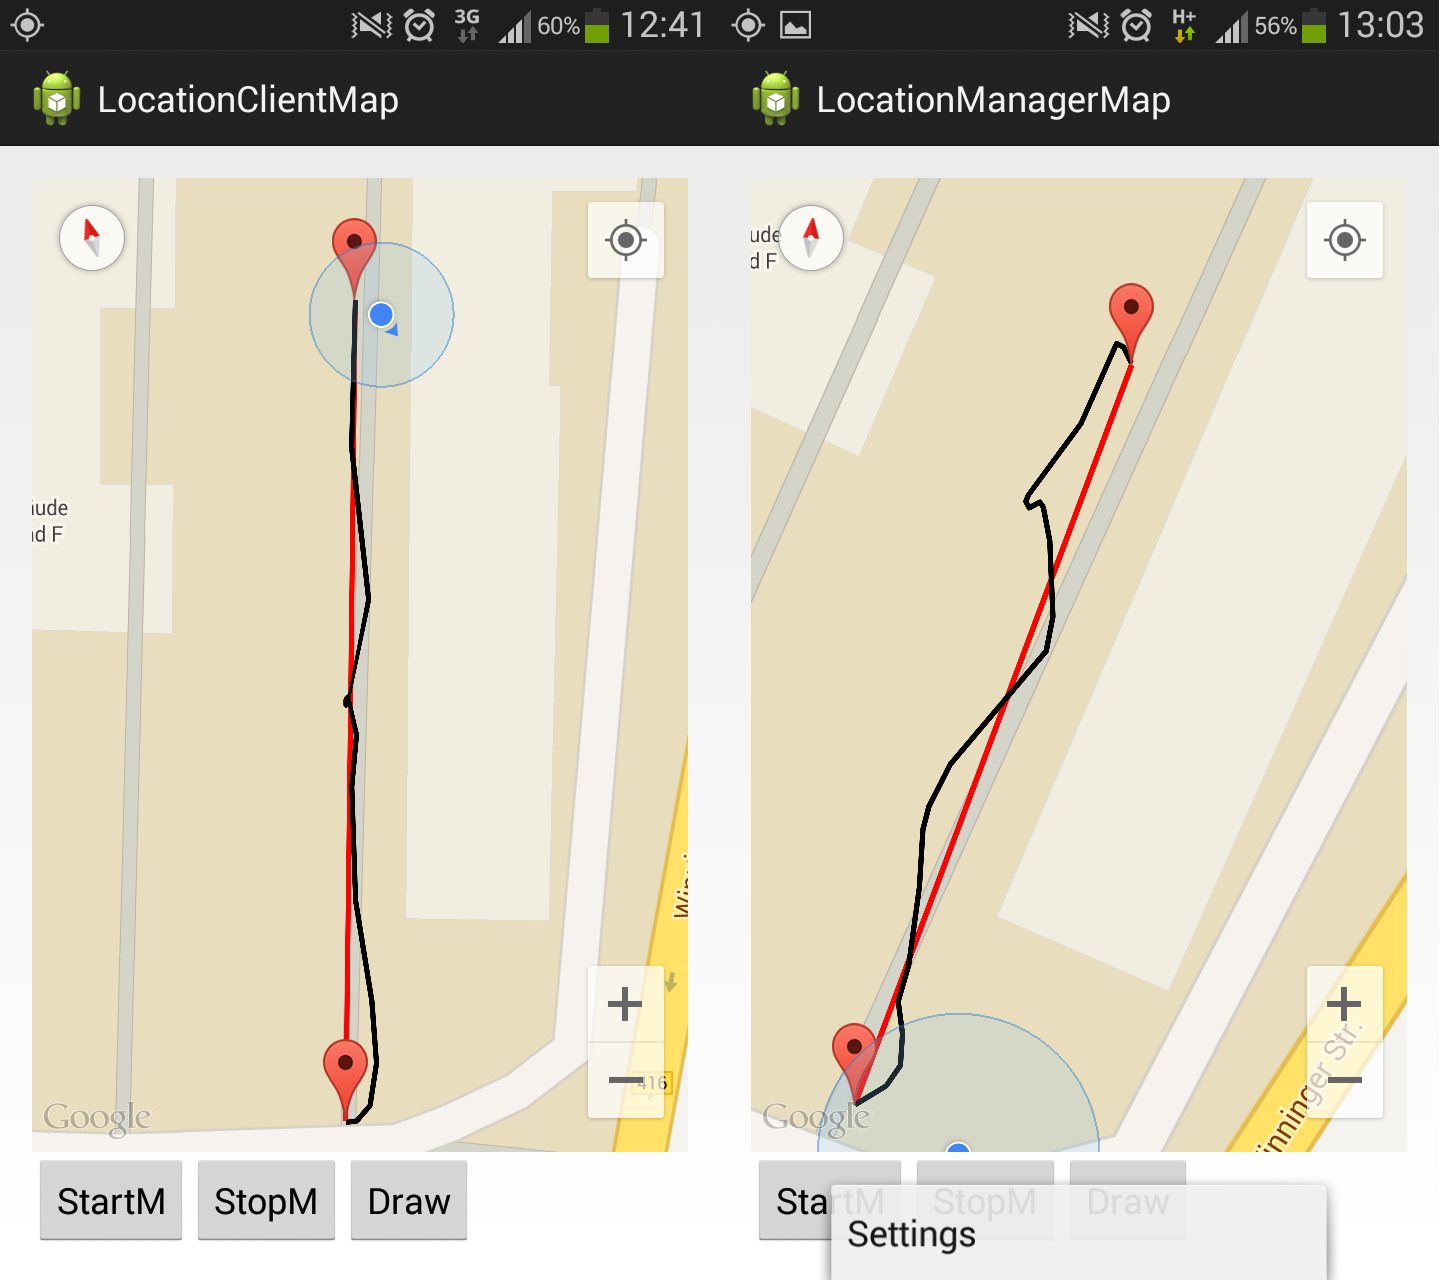
\includegraphics[width=0.48\textwidth]{4-Technische_Loesungen/4-1-Positionsermittlung/Data/Screenshot_2014-12-10-12-41-12_fuusion.png}
     \caption{Location Versuch 1}
     \label{fig: picLV1}
  \end{figure}

  \begin{figure}
    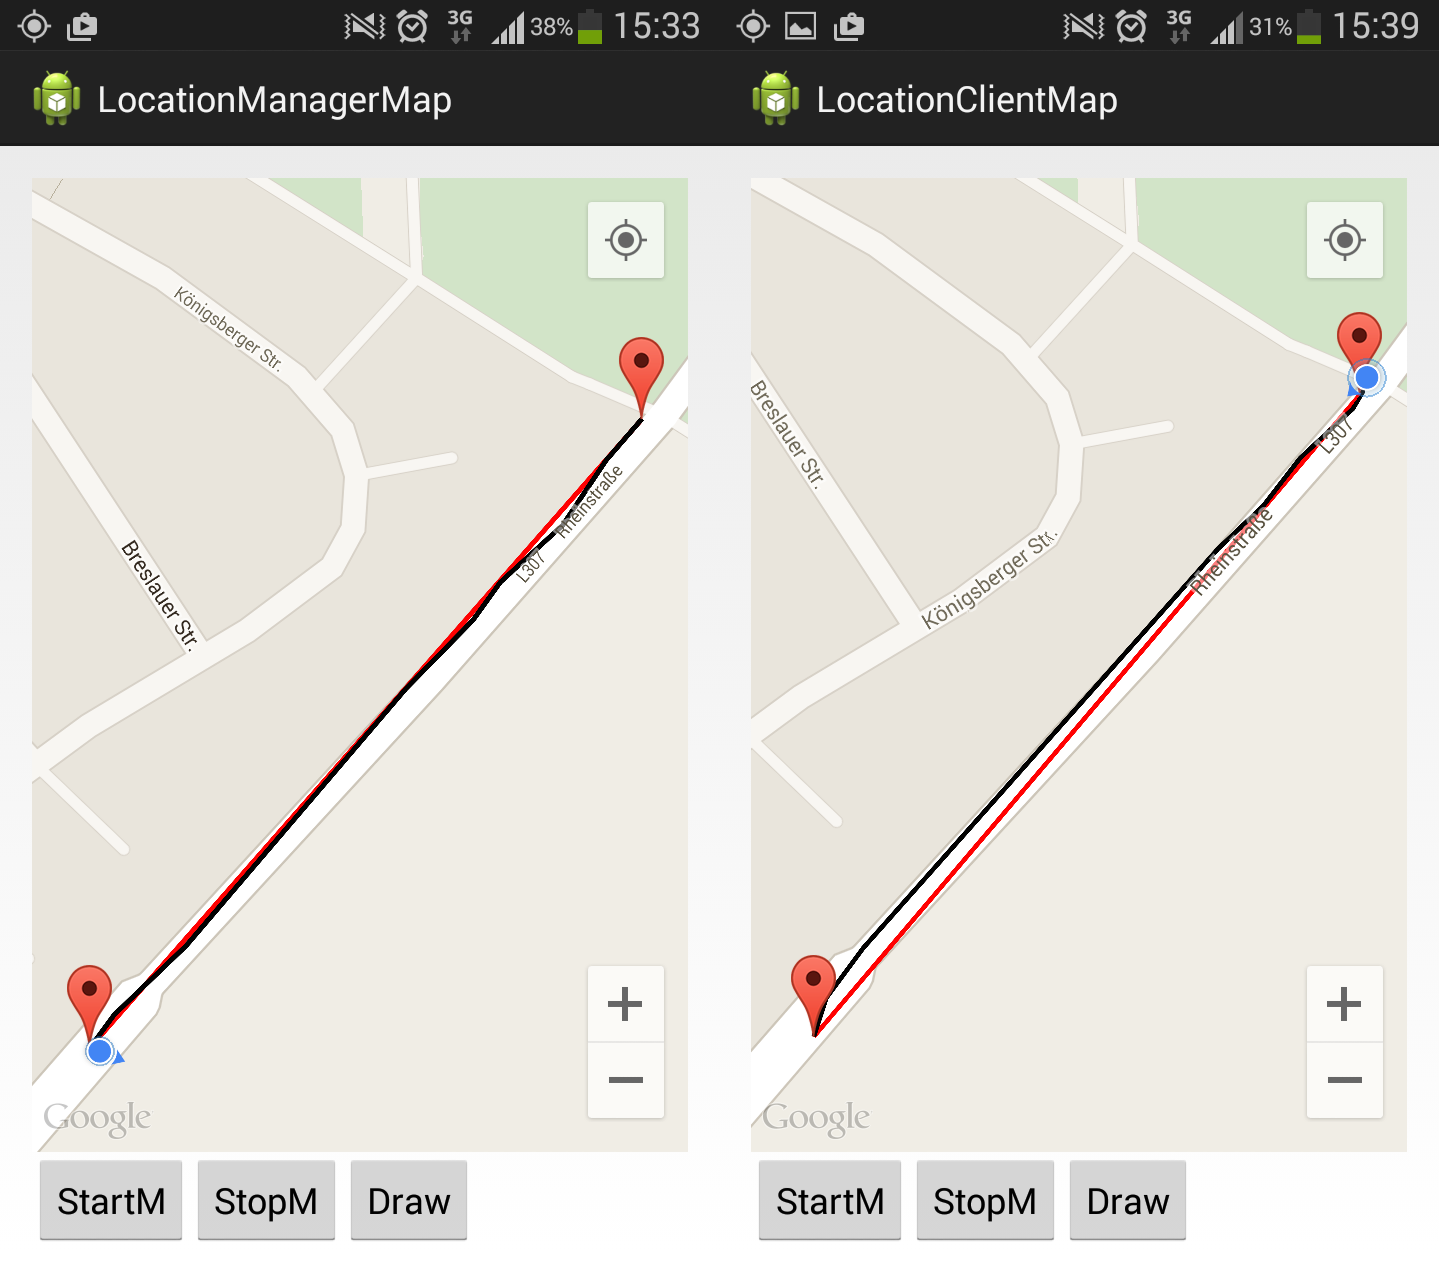
\includegraphics[width=0.48\textwidth]{4-Technische_Loesungen/4-1-Positionsermittlung/Data/Screenshot_2014-12-14-15-33-10_fuusion.png}
     \caption{Location Versuch 2}
     \label{fig: picLV2}
  \end{figure}
  
  
\subsection{Fazit}
Die Messdaten belegen, dass der LocationClient die minimal die besseren Ergebnisse liefert. Dies ist der Fall bei der Genauigkeit der
Sensordaten, als auch wei der grafischen Darstellung. Zweiteres ist ein wichtiger Faktor beim Umsetzten des Snakespiels. Die Unterschiede bei Updates pro Sekunde sind verschwindend gering und nicht eindeutig. Ein weiteres Faktor ist bereits, dass sich schon f�r die Kartenanzeige f�r GoogleMaps entschieden wurde. Da der LocationClient minimal die besseren Ergebnisse liefert und schon ein dienst von Google verwendet wird, wird zur Positionsermittlung in diesem Projekt der LocationClient verwendet.